
\documentclass[12pt, a4paper]{article}
\usepackage{fullpage}
\usepackage{graphicx}
\usepackage{wrapfig}
\usepackage{amsmath}
\usepackage{float}
\usepackage{listings}
\usepackage{lmodern}  % for bold teletype font
\usepackage{xcolor}   % for \textcolor

\definecolor{codegreen}{rgb}{0,0.6,0}
\definecolor{codegray}{rgb}{0.5,0.5,0.5}
\definecolor{codepurple}{rgb}{0.58,0,0.82}
\definecolor{backcolour}{rgb}{0.95,0.95,0.92}

\title{\textbf{EE2703 : Applied Programming Lab \\ Assignment 9}} % Title

\author{Potta Muni Asheesh \\ EE19B048} % Author name

\date{\today} % Date for the report

\begin{document}	
\lstset{
  language=Python,
  backgroundcolor=\color{backcolour},   
  commentstyle=\color{codegreen},
  keywordstyle=\color{magenta},
  numberstyle=\tiny\color{codegray},
  stringstyle=\color{codepurple},
  basicstyle=\ttfamily,
  breakatwhitespace=false,         
  breaklines=true,                 
  captionpos=b,                    
  keepspaces=true,                 
  %numbers=left,                    
  %numbersep=5pt,                  
  showspaces=false,                
  showstringspaces=false,
  showtabs=false,                  
  tabsize=2,
  columns=fullflexible,
  frame=single,
  postbreak=\mbox{\textcolor{red}{$\hookrightarrow$}\space},
}	
		
\maketitle % Insert the title, author and date

\section{Introduction}

In this assignment, the Discrete Fourier Transforms (DFTs) of varies function are computed using Fast Fourier Transform (FFT). FFT is an algorithm to compute the DFT of a function or signal in O(NlogN) time complexity. There are built-in functions in \texttt{numpy} to compute FFT and IFFT.

\section{DFT of a signal}

Consider a discrete-time signal $x[n]$ of length $N$, then it's DFT $X[k]$ is defined as

\begin{equation*}
X[k] = \sum_{n=0}^{N-1}x[n]exp\left(-j\frac{2\pi n}{N} k \right)
\end{equation*}

\section{Spectrum of $sin(5t)$}

Consider the signal $x(t) = sin(5t)$. We know that the expected spectrum of this signal is
\begin{equation*}
X(\omega) = j0.5\delta(\omega+5) - j0.5\delta(\omega-5)
\end{equation*}

If a sampling interval of $2\pi / 128$ is chosen and the continous time signal is sampled for 128 samples from $t = 0$. The spectrum obtained is.

\begin{lstlisting}
def ex1():
    t = np.linspace(0, 2*np.pi, 129)[:-1]
    x = np.sin(5*t)
    Y = fft(x)
    plt.figure()
    plt.subplot(2,1,1)
    plt.plot(np.abs(Y))
    plt.ylabel(r'$|X|$', size=16)
    plt.title(r'Spectrum of $x(t) = sin(5t)$')
    plt.grid(True)
    plt.subplot(2,1,2)
    plt.plot(np.unwrap(np.angle(Y)))
    plt.ylabel(r'$\angle X$', size=16)
    plt.xlabel(r'$k$', size=16)
    plt.grid(True)
\end{lstlisting}

\begin{figure}[H]
\centering
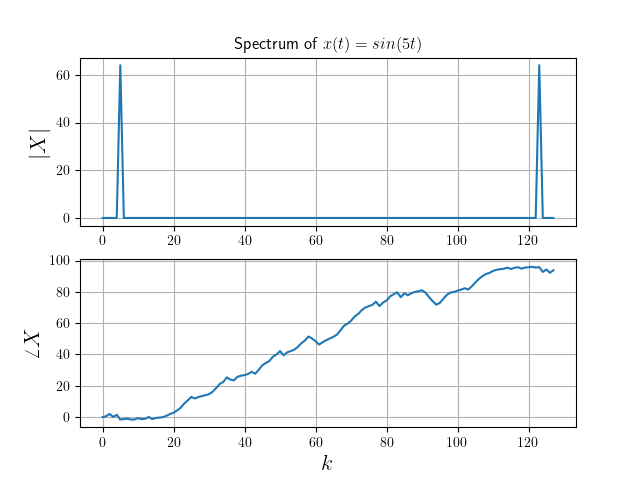
\includegraphics[width=0.8\textwidth]{ex1.png}
\end{figure}

There are some corrections which are needed to be done.

\begin{itemize}
\item DFT is the sampled version of DTFT over discrete-time angular frequency $[0, 2\pi )$. When trying to represent the continous time spectrum, the $\pi$ to $2\pi$ part of the spectrum should be shifted to the negative frequencies. This is done using \texttt{fftshift}.
\item The peaks are not of the appropriate height, there should be a scaling factor of 1/N.
\item The maximum continous time angular frequency is $\pi \times F_s = \pi \times N/2\pi = N/2$, where sampling frequency $F_s = N/2\pi$
\end{itemize}

After these corrections, the spectrum obtained is

\begin{lstlisting}
def q1():
    N = 128
    T = (2*np.pi)/N
    t = np.linspace(0, N*T, N+1)
    t = t[:-1]
    x = np.sin(5*t)
    x_spec = np.fft.fftshift(np.fft.fft(x))/N
    W = 2*np.pi/T
    w = np.linspace(-0.5*W, 0.5*W, N+1)
    w = w[:-1]
\end{lstlisting}

\begin{figure}[H]
\centering
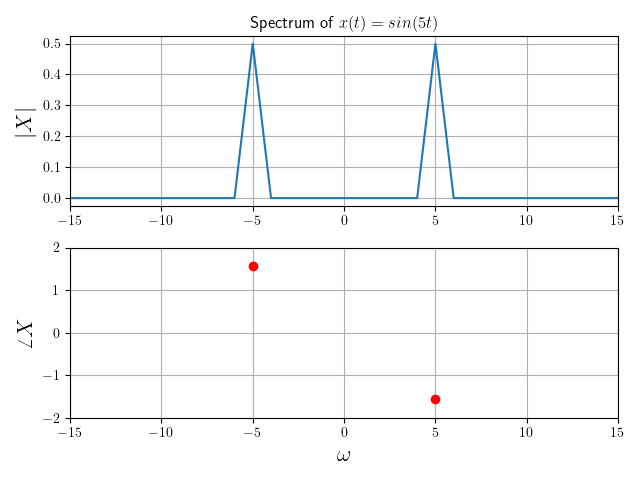
\includegraphics[width=0.8\textwidth]{q1sin.png}
\end{figure}

Here, only the phase of spectrum at frequencies at which the magnitude is $> 10^-3$ is indicated.

\section{Amplitude Modulated signal}

Consider an amplitude modulated signal,
\begin{equation*}
y(t) = (1 + 0.1cos(t))cos(10t)
\end{equation*}

This can be rewritten as,

\begin{equation*}
y(t) = cos(10t) + 0.05cos(9t) + 0.05cos(11t)
\end{equation*}

The expected spectrum is 
\begin{equation*}
Y(\omega) = 0.5\delta(\omega+10) + 0.5\delta(\omega-10) + 0.025\delta(\omega+9) + 0.025\delta(\omega-9) + 0.025\delta(\omega+11) + 0.025\delta(\omega-11)
\end{equation*}

The spectrum obtained, when sampled over an interval of $[0, 2\pi )$ at sampling frequency $F_s = 128/2\pi $, is

\begin{lstlisting}
def q1():
    N = 128
    T = (2*np.pi)/N
    t = np.linspace(0, N*T, N+1)
    t = t[:-1]
    y = (1 + 0.1*np.cos(t))*np.cos(10*t)
    y_spec = np.fft.fftshift(np.fft.fft(y))/N
    W = 2*np.pi/T
    w = np.linspace(-0.5*W, 0.5*W, N+1)
    w = w[:-1]
\end{lstlisting}

\begin{figure}[H]
\centering
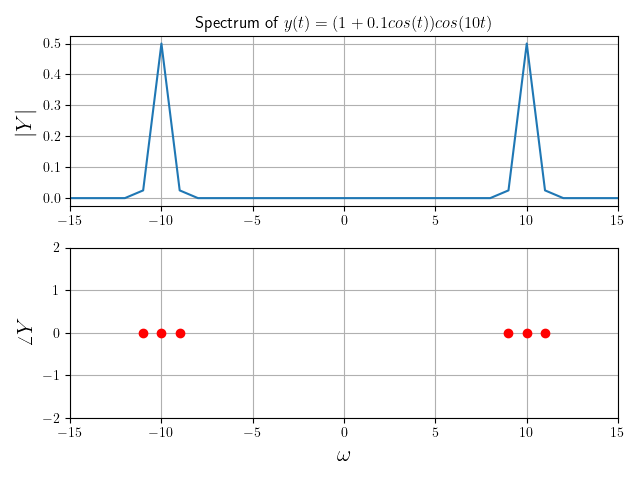
\includegraphics[width=0.8\textwidth]{q1cos.png}
\end{figure}

The small peaks at $\omega = 9, 11$ rads/s are mixed with the peak at $\omega = 10$ rads/s. In order to get better resolution spectrum, the sampled signal length should be increased without changing the sampling frequency.

When sampled over the interval of $[0, 8\pi)$ at the same sampling frequency, the spectrum obtained is

\begin{lstlisting}
def q1():
    N = 512
    T = (8*np.pi)/N
    t = np.linspace(0, N*T, N+1)
    t = t[:-1]
    y = (1 + 0.1*np.cos(t))*np.cos(10*t)
    y_spec = np.fft.fftshift(np.fft.fft(y))/N
    W = 2*np.pi/T
    w = np.linspace(-0.5*W, 0.5*W, N+1)
    w = w[:-1]
\end{lstlisting}

\begin{figure}[H]
\centering
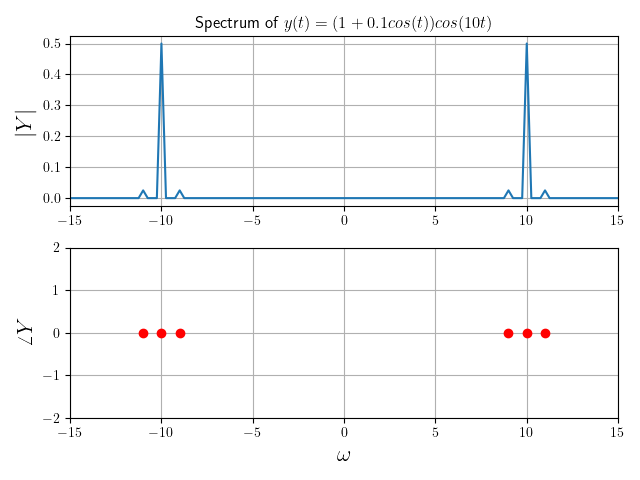
\includegraphics[width=0.8\textwidth]{q1cos1.png}
\end{figure}

Now, the spikes are clearly visible.

\section{Spectrum of $sin^3(t)$ and $cos^3(t)$}

Consider the signals

\begin{align*}
x(t) = sin^3(t) \\
y(t) = cos^3(t)
\end{align*}

These signals can be rewritten as

\begin{align*}
x(t) = \frac{3}{4}sin(t) - \frac{1}{4}sin(3t) \\
y(t) = \frac{3}{4}cos(t) + \frac{1}{4}cos(3t) \\
\end{align*}

When sampled over the interval $[0, 8\pi)$ at the sampling frequency $F_s = 128/2\pi$ Hz, the spectrum is obtained as

\begin{lstlisting}
def q2():
    N = 512
    T = (8*np.pi)/N
    t = np.linspace(0, 8*np.pi, N+1)
    t = t[:-1]
    x = np.sin(t)**3
    x_spec = np.fft.fftshift(np.fft.fft(x))/N
    y = np.cos(t)**3
    y_spec = np.fft.fftshift(np.fft.fft(y))/N
    W = 2*np.pi/T
    w = np.linspace(-0.5*W, 0.5*W, N+1)
    w = w[:-1]
\end{lstlisting}

\begin{figure}[H]
\centering
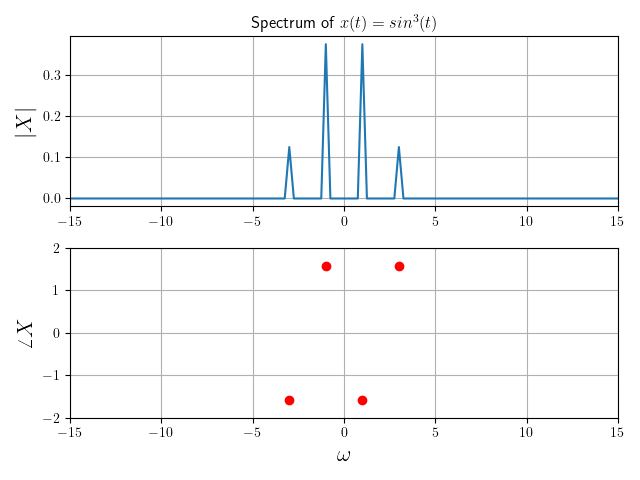
\includegraphics[width=0.8\textwidth]{q2sin.png}
\end{figure}

\begin{figure}[H]
\centering
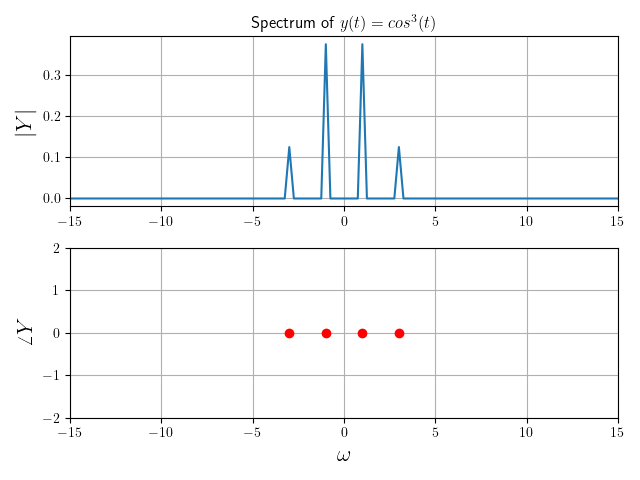
\includegraphics[width=0.8\textwidth]{q2cos.png}
\end{figure}

These plots are as expected.

\section{Frequency modulated signal}

Consider the signal,
\begin{equation*}
x(t) = cos(20t + 5cos(t))
\end{equation*}

When sampled over the time interval $[0, 8\pi)$ with sampling frequency $F_s = 128/2\pi$, the spectrum obtained is,

\begin{lstlisting}
def q3():
    N = 512
    T = (8*np.pi)/N
    t = np.linspace(0, 8*np.pi, N+1)
    t = t[:-1]
    x = np.cos(20*t + 5*np.cos(t))
    x_spec = np.fft.fftshift(np.fft.fft(x))/N
    W = 2*np.pi/T
    w = np.linspace(-0.5*W, 0.5*W, N+1)
    w = w[:-1]
\end{lstlisting}

\begin{figure}[H]
\centering
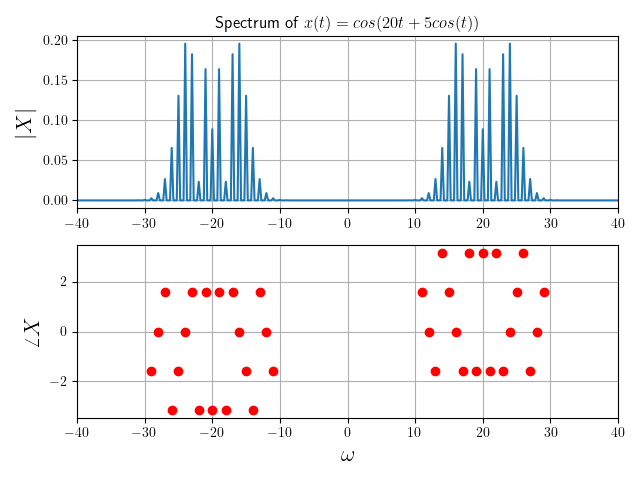
\includegraphics[width=0.8\textwidth]{q3.png}
\end{figure}

In frequency modulation, the information is distributed over a band of frequencies around 20 rads/s, where as in amplitude modualtion, it is not the case and most of the energy is with the carrier signal.

\section{Spectrum of Gaussian function}

Consider the Gaussian function,

\begin{equation*}
x(t) = e^{-t^2/2}
\end{equation*}

Analytically, the CTFT of Gaussian function is given as

\begin{equation*}
X(\omega) = \frac{1}{\sqrt{2\pi}}e^{-\omega^2/2}
\end{equation*}

A fixed sampling frequency of $128/2\pi$ Hz. When sampled over the time interval of $[-\pi, \pi)$, the spectrum obtained and the expected spectrum are shown below.

\begin{lstlisting}
def q4():
    N = 128 # number of samples
    T = (2*np.pi)/N # sampling time interval
    t = np.linspace(-0.5*N*T, 0.5*N*T, N+1)
    t = t[:-1]
    x = np.exp(-0.5*t*t)
    x_spec = np.fft.fftshift(np.fft.fft(np.fft.ifftshift(x)))*(1/N)
    W = 2*np.pi/T
    w = np.linspace(-0.5*W, 0.5*W, N+1)
    w = w[:-1]
\end{lstlisting}

\begin{figure}[H]
\centering
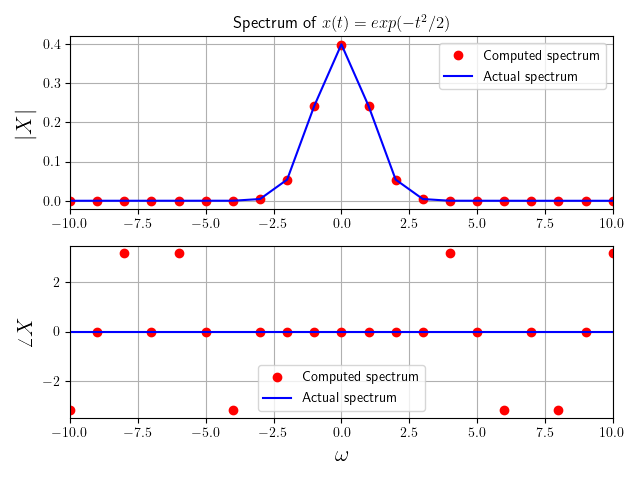
\includegraphics[width=0.8\textwidth]{q4_1.png}
\end{figure}

Here the maximum absolute error from the actual spectrum is 0.0006717929457629168

When sampled over the time interval $[-2\pi, 2\pi)$ at same sampling frequency, the spectrum obtained is

\begin{figure}[H]
\centering
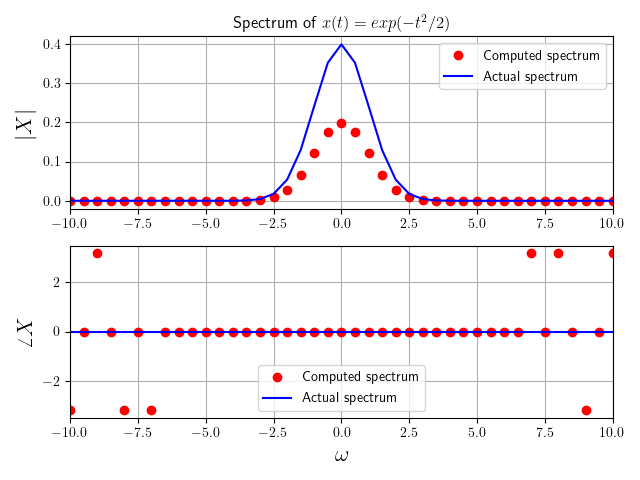
\includegraphics[width=0.8\textwidth]{q4_2.png}
\end{figure}

Here, the computed spectrum has clearly deviated from the actual spectrum. The deviation is due to scaling factor from the observation that the computed spectrum is about half of the actual spectrum.

This is confirmed when the time interval is increased $[-4\pi, 4\pi)$ and the spectrum obtained is 

\begin{figure}[H]
\centering
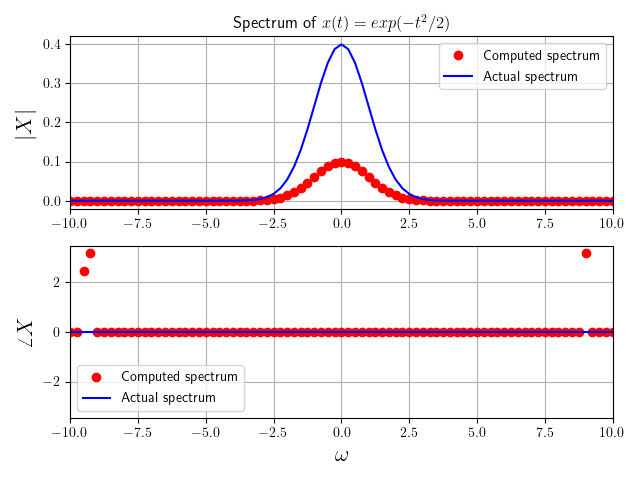
\includegraphics[width=0.8\textwidth]{q4_3.png}
\end{figure}

So, instead of taking the scaling factor as $1/N$, $1/(2\pi F_s)$ is considered, i.e; 1/(number of samples per $2\pi$ time). Then, the spectrum obtained when time interval considered is $[-2\pi, 2\pi)$, is.

\begin{lstlisting}
def q4():
    N = 256 # number of samples
    T = (4*np.pi)/N # sampling time interval
    t = np.linspace(-0.5*N*T, 0.5*N*T, N+1)
    t = t[:-1]
    x = np.exp(-0.5*t*t)
    x_spec = np.fft.fftshift(np.fft.fft(np.fft.ifftshift(x)))*(T/(2*np.pi))
    W = 2*np.pi/T
    w = np.linspace(-0.5*W, 0.5*W, N+1)
    w = w[:-1]
\end{lstlisting}

\begin{figure}[H]
\centering
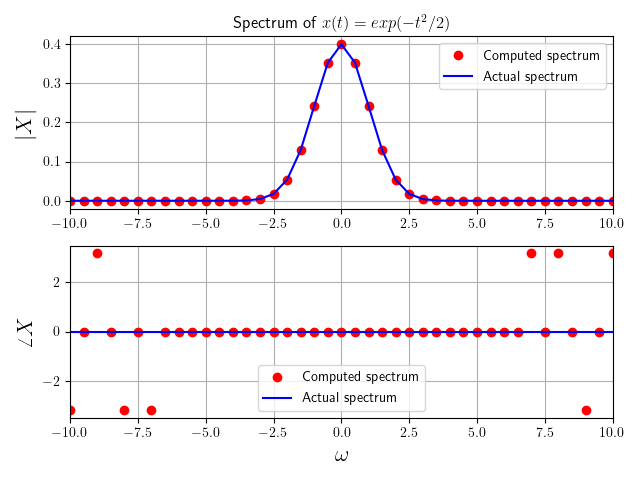
\includegraphics[width=0.8\textwidth]{q4_4.png}
\end{figure}

Here, the maximum absolute error from the actual spectrum is $1.3340406557205142 \times 10^{-10}$

Hence, it is observed that the scaling factor for non band-limited signals is not the same as that for band-limited signals.

\end{document} 
